%% ICAMAC 2026 --- IEEE Xplore conference (IEEEtran)
%% Overleaf: Menu -> Compiler -> pdfLaTeX. Recompile twice.
%% Blind CMT: comment \author{...} and uncomment \author{Anonymous authors}
%% Arabic (Table III): if missing glyphs, switch compiler to XeLaTeX.

\documentclass[conference]{IEEEtran}
\IEEEoverridecommandlockouts
\usepackage{cite}
\usepackage{amsmath,amssymb}
\usepackage{graphicx}
\usepackage{textcomp}
\usepackage{booktabs}
\usepackage{array}
\usepackage{url}
\usepackage{balance}
\usepackage{tikz}
\usetikzlibrary{arrows.meta,positioning}

\newcommand{\ar}[1]{#1}

\begin{document}

\title{SyNAPSE: Design and Security Audit of a Local-First Emotion-Aware AAC Platform}

\author{\IEEEauthorblockN{1\textsuperscript{st} Neha Vinod}
\IEEEauthorblockA{\textit{School of Engineering and IT}\\
\textit{Manipal Academy of Higher Education, Dubai Campus}\\
Dubai, UAE\\
neha.vinod@dxb.manipal.edu}
\and
\IEEEauthorblockN{2\textsuperscript{nd} Dr.\ Raja Varma Pamba}
\IEEEauthorblockA{\textit{School of Engineering and IT}\\
\textit{Manipal Academy of Higher Education, Dubai Campus}\\
Dubai, UAE\\
pamba.rajavarma@manipaldubai.com}}

% \author{Anonymous authors}

\maketitle

\begin{abstract}
Augmentative and Alternative Communication (AAC) systems have increasingly been paired with biometric emotion detection with role-based, multiple-stakeholder access, yet the access-control layer of the systems that are deployed is not as frequently audited as their machine-learning components. This paper presents a role-based access control (RBAC) audit of SyNAPSE, which is a local-first emotion-aware AAC system for children who are minimally verbal. Two distinct vulnerabilities surfaced while probing 42 protected REST endpoints out of a full API surface of 44 REST endpoints and 2 WebSocket channels across four user roles, which totaled 168 authenticated requests. First was a strict report-access rule that silently kept denying valid student and SEND-officer requests, and secondly a bug that caused authorization violations invisible to any logging pipeline built on the API by causing unauthorized probes to fail at the transport layer rather than returning a clean HTTP 403. Both of the vulnerabilities were fixed and verified, which raised the policy-correct outcome to 168/168 (100\%). By auditing each column of all 21 tables, we confirmed that there are no binary image or video blobs, satisfying UAE Federal Decree-Law No.~45 of 2021 through verifiable structure rather than policy language. To enhance this audit, we provide reproducible system-performance benchmarks (for PDF generation, WebSocket alerts, LLM-based card generation, and rule-based fallback in case the LLM card generation is slow or fails) alongside an emotion-detection test using 5{,}000 images from the public FER-2013 subset. Instead of publishing a single simplified result, we report a train-versus-test split comparison that fixes a potential data-contamination issue. The outcome is a code-verified breakdown of what is truly validated in a real deployed AAC system. This work contributes to software security and system architecture rather than an emotion-recognition accuracy claim.
\end{abstract}

\begin{IEEEkeywords}
role-based access control, software security audit, service-oriented architecture, augmentative and alternative communication, data minimization, local large language models, facial emotion recognition, neurodiversity
\end{IEEEkeywords}

\section{Introduction}
\IEEEPARstart{A}{ugmentative} and Alternative Communication (AAC) systems allow minimally verbal children, including many on the autism spectrum and those with cerebral palsy, to convey their needs and emotions through texts, symbols, or speech outputs. Commercially available AAC platforms usually use static vocabulary grids and cloud backends, which can complicate real-time emotion-aware adaptation and raise privacy concerns when the webcam frames are sent off the devices or uploaded to the cloud. Schools operating within inclusive-education frameworks additionally require tracking records for special-education-needs (SEND) reporting while maintaining minimal retention of biometric data.

Previous AAC and machine-learning prototypes usually addressed one concern at a time---either facial emotion recognition, or LLM-based phrase generation, or multi-role dashboards---rather than combining them with reproducible benchmarking in one deployable stack. SyNAPSE addresses these gaps directly, and this paper audits its own quantitative claims against the running codebase and benchmark artifacts, reporting the corrections and open gaps instead of only the intended behavior.

This study addresses the following research questions to evaluate the performance of SyNAPSE:
\begin{itemize}
  \item \textbf{RQ1:} Can an open-sourced platform that runs entirely locally be fast enough to hold a conversation flow with the individual using it, while also not persisting webcam frames (derived emotion labels may persist)?
  \item \textbf{RQ2:} Do login and user permissions successfully restrict users based on their school role across the pathways, and are security flaws detected during testing?
  \item \textbf{RQ3:} Which specific system component causes the most errors during testing---the LLM card generator, facial emotion recognition, or report access control?
\end{itemize}

The following summarizes the main contributions of the work:
\begin{itemize}
  \item We build an AAC system that runs completely on local devices and combines React~\cite{b16}, FastAPI~\cite{b15}, SQLite (21 tables), DeepFace~\cite{b6}, and Ollama~\cite{b10} \texttt{llama3}, while using a ruleset that ensures no images or webcam frames are saved permanently.
  \item After finding and fixing two important security issues during the code review, a security framework for four different user roles passed 168 access tests successfully.
  \item We provide a reproducible testing program that automatically creates spreadsheets that measure the speed of the system, overall security and reliability, and the accuracy of emotion detection.
  \item A double-check of the code was done to separate local test results from publicly available data tests. By reviewing 5{,}000 facial images from the public FER-2013 dataset, we identified and corrected an approximately 15-point train-contamination risk.
\end{itemize}

\section{Related Work}
\subsection{AAC Systems}
AAC can be unaided (gesture, sign, or facial expression) or aided (communication boards, speech-generating devices, tablet applications)~\cite{b1}. There is evidence that children with autism spectrum disorder (ASD) who are minimally verbal can show communication gains with the use of commercial aided systems such as Proloquo2Go, TouchChat, and LAMP Words for Life~\cite{b1,b2}. The most commonly adopted design basis for today's AAC boards is core-vocabulary systems centered around common high-frequency words (want, help, more, stop, yes, and no)~\cite{b3}. A survey by Holyfield \emph{et al.} indicated that the majority of publicly available AAC applications are based on a set of preprogrammed symbol hierarchies that need to be expertly configured by the user, and that none of these applications adapt the vocabulary to the user's current emotional state~\cite{b4}, which inspired the emotion-adaptive approach taken in this work.

\subsection{Facial Emotion Recognition}
The Facial Action Coding System developed by Ekman and Friesen is a system of seven emotion categories which are common to all cultures: happiness, sadness, anger, fear, disgust, surprise, and neutral. Recent years have seen significant progress in automatic facial emotion recognition through deep convolutional networks trained on large labelled corpora such as FER-2013, AffectNet, and CK+~\cite{b5}. An open-source Python framework called DeepFace, developed by Serengil and Ozpinar, offers a common API for face verification, recognition, and attribute-analysis tasks, such as emotion classification, and achieves competitive accuracy on common benchmarks~\cite{b6}. Monkaresi \emph{et al.} and Aslan \emph{et al.} have conducted classroom trials demonstrating emotion-aware learning technologies that enhance measures of student engagement~\cite{b7,b8}, but these systems were cloud-based and did not consider data-protection issues pertinent to SEND populations. Harms \emph{et al.} also point out that the distributions of facial expression in the autistic population might differ from the distributions found in the neurotypical training population, which any classroom-ready system must consider~\cite{b9}.

\subsection{Local LLMs for Contextual Generation}
Vocabulary generation and structured JSON output are among the tasks where instruction-tuned LLMs such as GPT-4, LLaMA~2, Mistral, and Llama~3 excel. This prototype uses Ollama \texttt{llama3}. The open-source runtime Ollama enables quantized LLMs to run locally on consumer hardware, without the need for a cloud API~\cite{b10}, and is suitable for educational use cases, such as UAE private schools, that prioritize data privacy and cost.

\subsection{KHDA SEND Framework and Privacy-by-Design}
The KHDA Inclusive Education Policy outlines a six-phase cycle of SEND~\cite{b11} that must be documented for each student: Identification, Assessment, Planning, Implementation, Monitoring, and Review. SyNAPSE draws on the Communication Matrix developed by Rowland that covers seven communication levels from pre-intentional behavior to abstract symbol use~\cite{b12}; the Matrix is an established instrument, and we do not claim a clinical validation of SyNAPSE. SyNAPSE is designed to adhere to Privacy by Design principles~\cite{b13} and to UAE Federal Decree-Law No.~45 of 2021 on Personal Data Protection~\cite{b14}, including purpose limitation and data minimization for biometric processing, as biometric data is required to be minimized, limited to the purpose for which it is collected, and limited in storage.

\subsection{Research Gap}
The literature review did not reveal any open-source AAC system that integrates local facial emotion detection with adaptive AAC generation, bilingual English--Arabic KHDA-aligned PDF reporting, four different roles for stakeholders, and environment-aware school--home alert routing, all in one privacy-preserving, locally deployable platform.

\subsection{Summary of Identified Gaps}
SyNAPSE is motivated by four gaps. First, there is no open-source AAC system that combines facial-expression recognition with emotion-adaptive generation of AAC cards. Second, none of the commercially available AAC tools provides bilingual English--Arabic PDF session reporting with a six-phase SEND assessment workflow. Third, current emotion-aware education tools lack the four roles required in a real inclusive-education deployment (student, teacher, caregiver, and SEND officer). Fourth, no single platform includes bilingual interface support, fully local inference, KHDA-aligned documentation, and school-to-home alert routing in one system.

\section{System Architecture}
\subsection{Design Principles}
\textbf{Local-first:} DeepFace and Ollama are implemented on the same device as the API and they do not rely on an external SaaS service. \textbf{Data minimization:} \texttt{EmotionLog} does not contain any image or video field, so it only has \texttt{emotion\_label}, confidence score, intensity, and timestamp. \textbf{Graceful degradation:} If the LLM's output failed or it takes too much time, it does not generate an empty AAC board but instead loads a rule-based card template. Foreign keys are limited to child--teacher--caregiver relationships and gate each router (role separation). Local-first execution is also an attack-surface reduction: the remaining attack surface is the REST/WebSocket boundary that is being audited; there is no third-party inference API key, no child data in transit to SaaS inferences, and no external credential whose compromise would expose the protected data.

\begin{figure}[!t]
\centering
\resizebox{\columnwidth}{!}{%
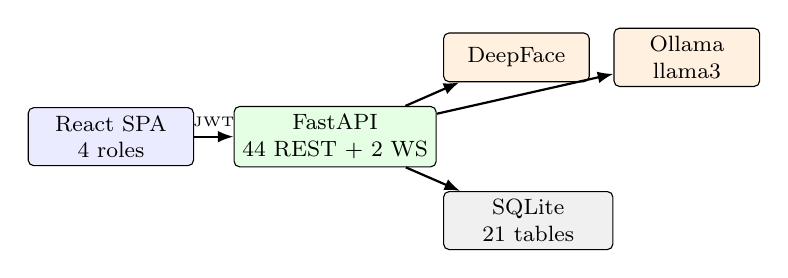
\begin{tikzpicture}[
  font=\footnotesize,
  box/.style={draw, rounded corners=2pt, align=center, minimum height=0.62cm, inner sep=3pt},
  arr/.style={-{Latex[length=2mm]}, thick}
]
\node[box, fill=blue!8, minimum width=2.1cm] (ui) {React SPA\\4 roles};
\node[box, fill=green!10, minimum width=2.5cm, right=0.5cm of ui] (api) {FastAPI\\44 REST + 2 WS};
\node[box, fill=orange!12, minimum width=1.85cm, above right=0.3cm and 0.08cm of api] (df) {DeepFace};
\node[box, fill=orange!12, minimum width=1.85cm, right=0.3cm of df] (oll) {Ollama\\llama3};
\node[box, fill=gray!12, minimum width=2.15cm, below right=0.3cm and 0.08cm of api] (db) {SQLite\\21 tables};
\draw[arr] (ui) -- node[above]{\tiny JWT} (api);
\draw[arr] (api) -- (df);
\draw[arr] (api) -- (oll);
\draw[arr] (api) -- (db);
\end{tikzpicture}}
\caption{Local-first SyNAPSE architecture. Webcam frames are processed in memory and only derived affect labels persist to SQLite.}
\label{fig:arch}
\end{figure}

\subsection{Session and Alert Pipeline}
The capture of emotions is not by continuous polling but is triggered by the user. \texttt{POST /api/emotion/detect} will resize each image frame to no more than 320\,px, use an OpenCV detector backend, run DeepFace, add an \texttt{EmotionLog} row, and check if there is an alert condition if the predicted emotion is in a configurable set (default: sad, angry, fear, disgust, \ldots) and if the confidence exceeds the configurable threshold (default: 0.35). Finally, \texttt{POST /api/cards/generate} queries Ollama (120\,s timeout) and then generates a 16-card board.

\begin{figure}[!t]
\centering
\resizebox{\columnwidth}{!}{%
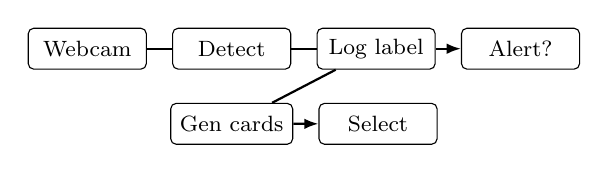
\begin{tikzpicture}[
  font=\footnotesize,
  proc/.style={draw, rounded corners=2pt, align=center, minimum width=1.5cm, minimum height=0.52cm},
  arr/.style={-{Latex[length=1.8mm]}, thick}
]
\node[proc] (cam) {Webcam};
\node[proc, right=0.32cm of cam] (det) {Detect};
\node[proc, right=0.32cm of det] (log) {Log label};
\node[proc, right=0.32cm of log] (alt) {Alert?};
\node[proc, below=0.42cm of det] (gen) {Gen cards};
\node[proc, right=0.32cm of gen] (sel) {Select};
\draw[arr] (cam)--(det)--(log)--(alt);
\draw[arr] (log)--(gen)--(sel);
\end{tikzpicture}}
\caption{On-demand emotion detection, zero-retention logging, optional WebSocket alert, and adaptive card generation.}
\label{fig:pipe}
\end{figure}

\subsection{Alert and Preprocessing Rules}
Alert triggering uses the cautious-emotion set $\{\mathrm{sad},\mathrm{angry},\mathrm{fear},\mathrm{disgust},\mathrm{distress},\mathrm{scared},\mathrm{frustrated}\}$ with minimum alert confidence of 0.35 and an alert cooldown of 45 seconds to reduce caregiver notification fatigue. DeepFace preprocessing (\texttt{deepface\_service.py}): frames are limited to 320\,px on the longest side, cropped with a Haar-cascade face detector, histogram-equalized, and resized to 224\,px when the crop is small. Checks are performed before DeepFace inference to reject a placeholder/blank image, and a \texttt{threading.Lock} is used to serialize concurrent calls to DeepFace. The seven DeepFace classes $\{\mathrm{happy},\mathrm{sad},\mathrm{angry},\mathrm{fear},\mathrm{disgust},\mathrm{surprise},\mathrm{neutral}\}$ are the allowed output labels.

\subsection{Technology Stack}
\begin{table}[!t]
\caption{Technology stack (deployed prototype).}
\label{tab:I}
\centering
\small
\begin{tabular}{@{}ll@{}}
\toprule
\textbf{Layer} & \textbf{Choice} \\
\midrule
Frontend & React 18, Vite, TailwindCSS \\
API & FastAPI, Uvicorn, python-jose JWT \\
Persistence & SQLite, SQLAlchemy (21 tables) \\
Expression & DeepFace, OpenCV detector, 320\,px cap \\
LLM & Ollama \texttt{llama3}, JSON parse + rule fallback \\
Reports & ReportLab (A4 PDF) \\
Realtime & \texttt{/ws/session/\{id\}}, \texttt{/ws/alerts} \\
\bottomrule
\end{tabular}
\end{table}

\section{Implementation}
\subsection{API Surface and RBAC}
There are 44 REST endpoints (11 routers totaling 42 routes, plus \texttt{/} and \texttt{/health}) in SyNAPSE and 2 WebSocket channels (46 surfaces in total) (Table~\ref{tab:II}). The roles are: student, teacher, caregiver, and send officer. Students are bound to their own child profile; teachers/caregivers are scoped through foreign keys; and SEND officers can access assessment and school-reporting dashboards.

\begin{table}[!t]
\caption{REST endpoint counts by router (WebSockets counted separately).}
\label{tab:II}
\centering
\small
\begin{tabular}{@{}lcr@{}}
\toprule
\textbf{Router} & \textbf{Prefix} & \textbf{\#} \\
\midrule
auth & \texttt{/auth} & 3 \\
children & \texttt{/api/children} & 4 \\
sessions & \texttt{/api/sessions} & 5 \\
emotion & \texttt{/api/emotion} & 1 \\
cards & \texttt{/api/cards} & 2 \\
assessments & \texttt{/api/assessments} & 6 \\
reports & \texttt{/api/reports} & 7 \\
send & \texttt{/api/send} & 2 \\
teacher & \texttt{/teacher} & 9 \\
alerts & \texttt{/api/alerts} & 2 \\
support & \texttt{/api/support} & 1 \\
main & \texttt{/}, \texttt{/health} & 2 \\
\bottomrule
\end{tabular}
\end{table}

\subsection{AAC Card Model}
The card-service program returns precisely 16 cards per board, with 8 cards showing the core-vocabulary symbols that are available in both languages, 4 cards that match the detected emotion, and 4 cards that represent the topic returned by the LLM if there are at least six valid LLM topic labels returned, or drawn from the deterministic fallback otherwise. Card selections remain with the emotion at the time of selection and complement session analytics. The topics that were benchmarked for LLM generation: school, home, play, food, feelings, body.

\begin{table}[!t]
\caption{The eight fixed bilingual core-vocabulary cards.}
\label{tab:III}
\centering
\small
\begin{tabular}{@{}ll@{}}
\toprule
\textbf{English} & \textbf{Arabic} \\
\midrule
I want & \ar{????} \\
Stop & \ar{????} \\
More & \ar{??????} \\
All done & \ar{?????} \\
I need help & \ar{????? ??????} \\
Yes & \ar{???} \\
No & \ar{??} \\
Wait & \ar{?????} \\
\bottomrule
\end{tabular}
\end{table}

\subsection{Database Schema}
These are the 21 SQLite tables: users, children, sessions, emotion\_logs, card\_selections, emotion\_alerts, assessments, routine\_templates, routine\_steps, sensory\_profiles, break\_activities, break\_logs, reward\_goals, reward\_events, badges, video\_models, self\_reports, display\_preferences, shared\_notes, calm\_corner\_sessions, and pre\_event\_plans. A column-by-column examination of all 21 tables confirmed that there are no table rows containing raw image or video binaries, and the only field containing a string URL reference to video content is \texttt{video\_models.url}, which points to media content that is hosted elsewhere; \texttt{emotion\_logs} contains no raw images or videos, only the derived fields \texttt{emotion\_label}, confidence, and intensity.

\subsection{Evaluation Accounts}
Benchmarks were executed against five seeded development accounts spanning all four roles (Table~\ref{tab:IV}), used only for local, non-production testing.

\begin{table}[!t]
\caption{Seeded development accounts used for benchmarking.}
\label{tab:IV}
\centering
\small
\begin{tabular}{@{}lll@{}}
\toprule
\textbf{Username} & \textbf{Role} & \textbf{Full name (fictional)} \\
\midrule
student & student & Ahmed Al Mansoori \\
teacher & teacher & Ms.\ Sarah Ahmed \\
teacher2 & teacher & Mr.\ James Wilson \\
caregiver & caregiver & Fatima Al Rashidi \\
sendofficer & send\_officer & Dr.\ Khalid Al Mansoori \\
\bottomrule
\end{tabular}
\end{table}

\section{Evaluation Methodology}
Eight benchmark scripts are placed under \texttt{synapse/tests/evaluation} that generate reproducible CSV artifacts in the \texttt{results/} folder for PDF generation, LLM card generation, WebSocket alert latency, LLM fallback triggering, role-access control, alert-threshold sensitivity, emotion-detection accuracy, and functional coverage (Table~\ref{tab:V}).

\begin{table}[!t]
\caption{Benchmark script inventory and CSV outputs.}
\label{tab:V}
\centering
\scriptsize
\begin{tabular}{@{}ll@{}}
\toprule
\textbf{Benchmark script} & \textbf{Output CSV} \\
\midrule
\texttt{bench\_pdf\_generation.py} & \texttt{pdf\_generation\_benchmark.csv} \\
\texttt{bench\_llm\_card\_generation.py} & \texttt{llm\_card\_generation\_benchmark.csv} \\
\texttt{bench\_websocket\_latency.py} & \texttt{websocket\_latency.csv} \\
\texttt{bench\_fallback\_trigger\_rate.py} & \texttt{fallback\_trigger\_rate.csv} \\
\texttt{bench\_emotion\_detection\_accuracy.py} & \texttt{emotion\_detection\_accuracy.csv} \\
\texttt{bench\_alert\_precision\_recall.py} & \texttt{alert\_precision\_recall.csv} \\
\texttt{bench\_role\_access\_matrix.py} & \texttt{role\_access\_matrix.csv} \\
\texttt{bench\_functional\_coverage.py} & \texttt{functional\_test\_coverage.csv} \\
\bottomrule
\end{tabular}
\end{table}

A pytest suite (Table~\ref{tab:VI}, 13 tests) includes tests for the emotion pipeline, authentication, and RBAC, while a per-endpoint coverage inventory (\texttt{functional\_test\_coverage.csv}, 46 rows) shows the mapping of tests per endpoint, but only 3 of 46 surfaces are currently covered by the pytest suite, with others remaining open items as of this draft.

\begin{table}[!t]
\caption{Automated pytest suite (13 tests total).}
\label{tab:VI}
\centering
\small
\begin{tabular}{@{}llp{3.3cm}@{}}
\toprule
\textbf{Test file} & \textbf{\#} & \textbf{Covers} \\
\midrule
\texttt{test\_auth.py} & 4 & login, wrong password, protected route, valid token \\
\texttt{test\_rbac.py} & 7 & report access $\times$4 roles; teacher 403 $\times$3 roles \\
\texttt{test\_emotion\_pipeline.py} & 2 & real face label; blank image handling \\
\bottomrule
\end{tabular}
\end{table}

\textbf{Hardware:} local Ollama, CPU-only inference, and a single developer workstation. \textbf{Validation issues:} single-machine measurement and seeded data limit external validity. The emotion-recognition integration check uses held-out test-split crops from the public FER-2013 dataset (5{,}000 images, 7 emotion classes, with naturally low counts in the disgust class at $n{=}109$). The audit and fixes were carried out by the developers of the platform; confirmation bias cannot be ruled out despite code-based reporting discipline.

\section{Results}
\subsection{Latency and Reliability}
Data from the current benchmark CSV outputs have been used to produce verified statistics, which are reported in Table~\ref{tab:VII}. LLM card-generation latency is right-skewed (median 7.25\,s is significantly lower than the mean of 10.90\,s), indicating that generation occasionally takes a long time rather than a strict bimodal cold-start/steady-state split. There were no fallbacks due to a timeout in this run; all 22 fallbacks (18.3\% out of 120 trials) were triggered by malformed JSON output.

\begin{table}[!t]
\caption{Performance benchmarks (pilot-scale, $n{=}30$--36; not load-tested at production scale).}
\label{tab:VII}
\centering
\small
\begin{tabular}{@{}lrrrr@{}}
\toprule
\textbf{Metric} & \textbf{$n$} & \textbf{Mean} & \textbf{Median} & \textbf{Max} \\
\midrule
PDF generation (s) & 30 & 0.317 & 0.199 & 1.010 \\
LLM card gen.\ (s) & 36 & 10.90 & 7.25 & 36.18 \\
WebSocket alert (s) & 30 & 0.724 & 0.698 & 1.233 \\
\bottomrule
\end{tabular}
\end{table}

\subsection{Role-Based Access Control}
\label{sec:rbac}
The deployed API had 168 authenticated requests (4 roles $\times$ 42 protected endpoint patterns) made to it. Two corrective fixes found during audit and verified with the latest benchmark run resulted in all 168 (100\%) matching the expected policy. Before the fixes, 10 of 168 probes failed: 4 were a genuine over-restrictive denial on session report/PDF routes, and 6 were routes on the teacher dashboard returning a transport-level status 0 (as opposed to a clean 403 for unauthorized roles).

\begin{table}[!t]
\caption{Role-based access control audit outcome.}
\label{tab:VIII}
\centering
\small
\begin{tabular}{@{}p{2.1cm}p{5.5cm}@{}}
\toprule
\textbf{Check} & \textbf{Result} \\
\midrule
Total probes & 168 (4 roles $\times$ 42 protected patterns) \\
Policy-correct & 168 (100\%) \\
Fix A & \texttt{reports\_router.py}: student/SEND-officer report access (was returning 403, now returns 200) \\
Fix B & \texttt{teacher\_router.py}: shadow bug causing status-0 transport errors on unauthorized probes; now returns clean 403 \\
\bottomrule
\end{tabular}
\end{table}

\subsection{Security Impact of Found Vulnerabilities and Threat Model}
Both findings are described under a role-confusion threat model where an actor who has an authenticated account but lower privilege (e.g., student or caregiver) tries to access a route scoped to another of the four roles (student, teacher, caregiver, SEND officer---there is no administrator role). Fix~A was a false-negative denial, showing that the ACL logic had not been exercised against its own role matrix. The more security-relevant result is the variable-shadowing bug, which caused the teacher-router program to return a transport-level status 0 \emph{instead of} HTTP 403 when an unauthorized role tried to access. After the fix, those probes return a clean 403. As far as the client or logging pipeline is concerned, a status-0 transport failure is indistinguishable from a network failure, so monitoring built on the API would not have logged these as authorization denials. This is not a confirmed data exposure: the route handler still rejected the call before returning data. Even so, the denials were not visible to audit logging, and the paper's compliance argument (UAE Federal Decree-Law No.~45 of 2021~\cite{b14}) relies on verifiable enforcement, not policy language. We take this as the main security contribution of the paper: a boundary defect that functional tests would not have recorded as a clean denial.

\subsection{Emotion Recognition Pilot (Preliminary Integration Check)}
This subsection does not claim to validate the paper's main contribution, RBAC (Section~\ref{sec:rbac}), but rather reports on a preliminary integration check of the emotion-detection pipeline. The fixtures are $48\times48$ FER-2013 crops (Goodfellow \emph{et al.}, 2013) from HuggingFace \texttt{gulsunnciftci/fer2013}. The accuracy of an initial $n{=}5000$ train-split was 62.4\%, but the expression model used by DeepFace is commonly trained with FER-2013, which may contaminate train-split tests, so we re-ran on the held-out test split published below. The natural imbalance of the test split is only 109 validated disgust crops compared with approximately 791 to 821 for the other six classes, which was not made up synthetically. No claim of SOTA-FER or clinical efficacy is being made.

\begin{table}[!t]
\caption{FER-2013 held-out test-split per-class results ($n{=}5000$; disgust is rare in the test split).}
\label{tab:IX}
\centering
\small
\begin{tabular}{@{}lrrrr@{}}
\toprule
\textbf{Class} & \textbf{$n$} & \textbf{Correct} & \textbf{Recall} & \textbf{F1} \\
\midrule
Angry & 821 & 307 & 0.374 & 0.418 \\
Disgust & 109 & 18 & 0.165 & 0.250 \\
Fear & 820 & 248 & 0.302 & 0.310 \\
Happy & 820 & 622 & 0.759 & 0.697 \\
Neutral & 820 & 447 & 0.545 & 0.462 \\
Sad & 819 & 325 & 0.397 & 0.375 \\
Surprise & 791 & 400 & 0.506 & 0.602 \\
\bottomrule
\end{tabular}
\end{table}

Overall top-1 accuracy on the held-out test split is $2367/5000 = 47.3\%$, macro-F1 $= 0.445$ (Table~\ref{tab:IX}), lowest among the harder classes (recall 0.302--0.374) and highest for happy (0.759). Disgust is the weakest (recall 0.165), consistent with it also being the rarest class in the test split.

\begin{table}[!t]
\caption{Train-split versus held-out test-split accuracy at matched $n{=}5000$, confirming a train-contamination effect of approximately 15 points; we report the test-split result as the paper's figure.}
\label{tab:X}
\centering
\small
\begin{tabular}{@{}lccc@{}}
\toprule
\textbf{FER-2013 split} & \textbf{$n$} & \textbf{Top-1 acc.} & \textbf{Macro-F1} \\
\midrule
Train (risk) & 5000 & 62.4\% & 0.610 \\
Test (reported) & 5000 & 47.3\% & 0.445 \\
\bottomrule
\end{tabular}
\end{table}

With this 15-point gap, evaluating on the train split is not measuring generalisation so much as memorisation risk. The reported result is only the held-out test result (47.3\%); Table~\ref{tab:X} is retained as a transparency check.

\subsection{Alert Threshold Sensitivity}
The precision and recall of the distress-alert trigger are given for three levels of confidence in Table~\ref{tab:XI} for the same set of 12 frames. The point of 0.35 is near the edge of the precision--recall trade-off in this small sample; precision is perfect at all three thresholds tested (no false alarms) and recall is 0.833 at 0.25--0.35. Frames f002 and f010 are missed at every tested threshold---both predicted `neutral' rather than a cautious label.

\begin{table}[!t]
\caption{Alert-threshold sensitivity ($n{=}12$ frames per threshold; pilot-scale; not re-run on the $n{=}5000$ FER-2013 test set).}
\label{tab:XI}
\centering
\small
\begin{tabular}{@{}lccc@{}}
\toprule
\textbf{Threshold} & \textbf{Precision} & \textbf{Recall} & \textbf{TP/FN/FP} \\
\midrule
0.25 & 1.000 & 0.833 & 10 / 2 / 0 \\
0.35 (default) & 1.000 & 0.833 & 10 / 2 / 0 \\
0.45 & 1.000 & 0.750 & 9 / 3 / 0 \\
\bottomrule
\end{tabular}
\end{table}

\section{Discussion}
Validated strengths include: PDF generation and WebSocket alerts are both comfortably within interactive latency budgets for a classroom. The rule-based LLM fallback can reliably avoid an empty AAC board when generation fails. After two RBAC bugs were found and corrected, RBAC enforces role separation correctly over all 168 probes.

Open risks: the train-split figure (62.4\%) is a contamination check only and cannot be considered a performance result, as DeepFace's classifier might be trained on FER-2013. Accuracy on the held-out FER-2013 test split (47.3\%, macro-F1 0.445) is an integration check, not a validated claim. FER-2013 is not a neurodivergent-population dataset; there are known variations in facial expression among autistic people~\cite{b9}. Modest accuracy is expected for an unmodified DeepFace backend. LLM card-generation latency (median 7.25\,s, max 36.18\,s) would be worth exploring for warm-up behavior. Per-endpoint automated coverage remains limited: only 3 of 46 API surfaces have a direct pytest mapping.

\section{Scope Limits}
To avoid overstatement, we clearly do not claim the following: state-of-the-art facial emotion recognition; continuous 2\,fps webcam polling (capture triggered by the user only); continuous background monitoring of children; or validated clinical/educational efficacy. This system has not yet been tested on children in the classroom and is not ready for deployment without further testing and ethics approval.

\textbf{AI disclosure:} The authors used Perplexity, Claude, and Grammarly to assist in drafting portions of the manuscript (introduction, discussion, and conclusion), in accordance with IEEE/ICAMAC policy on AI-generated content.

\textbf{Topic alignment:} This paper's main contribution is a software-security audit (RBAC vulnerability discovery and correction) and a service-oriented systems architecture, in line with ICAMAC Software Security and Software Architectures tracks; data-minimisation verification aligns with Ethics in AI. Facial expression detection is not featured as an essential novel element of the paper, but rather as a built-in, preliminary test, and is not a main finding of the paper.

\section{Conclusion}
SyNAPSE provides a local-first, emotion-aware, reproducibly measured AAC architecture combining DeepFace, Ollama \texttt{llama3}, and FastAPI with multi-stakeholder school workflows. Verified results include PDF/WebSocket latency, LLM timing and fallback behaviour, and 100\% (168/168) RBAC correctness following an audit which identified and fixed two true access-control bugs. With the held-out test split ($n{=}5000$) of FER-2013, the accuracy achieved for the emotion-recognition task is 47.3\% (macro-F1 is 0.445), and the result of a matched train-split is 62.4\%, highlighting the importance of held-out evaluation for a non-core benchmark.

\balance
\begin{thebibliography}{16}
\bibitem{b1} American Speech-Language-Hearing Association, ``Augmentative and Alternative Communication (AAC),'' 2024.
\bibitem{b2} D.~R. Beukelman and P.~Mirenda, \emph{Augmentative and Alternative Communication: Supporting Children and Adults with Complex Communication Needs}, 4th~ed. Baltimore, MD: Paul H.\ Brookes Publishing, 2013.
\bibitem{b3} J.~Light and D.~McNaughton, ``The changing face of augmentative and alternative communication: Past, present, and future challenges,'' \emph{Augmentative and Alternative Communication}, vol.~28, no.~4, pp.~243--246, Dec.~2012.
\bibitem{b4} C.~Holyfield, J.~Caron, and J.~Light, ``Programing AAC just-in-time for beginning communicators: The process,'' \emph{Augmentative and Alternative Communication}, vol.~35, no.~4, pp.~210--222, Oct.~2019.
\bibitem{b5} I.~J. Goodfellow \emph{et al.}, ``Challenges in representation learning: A report on three machine learning contests,'' arXiv:1307.0414, Jul.~2013.
\bibitem{b6} S.~I. Serengil and A.~Ozpinar, ``HyperExtended LightFace: A facial attribute analysis framework,'' in \emph{2021 Int.\ Conf.\ on Engineering and Emerging Technologies (ICEET)}, Oct.~2021.
\bibitem{b7} H.~Monkaresi, N.~Bosch, R.~A. Calvo, and S.~K. D'Mello, ``Automated detection of engagement using video-based estimation of facial expressions and heart rate,'' \emph{IEEE Trans.\ Affective Computing}, vol.~8, no.~1, pp.~15--28, Jan.~2017.
\bibitem{b8} S.~Aslan \emph{et al.}, ``Investigating the impact of a real-time, multimodal student engagement analytics technology in authentic classrooms,'' in \emph{Proc.\ 2019 CHI Conf.\ on Human Factors in Computing Systems}, 2019.
\bibitem{b9} M.~B. Harms, A.~Martin, and G.~L. Wallace, ``Facial emotion recognition in autism spectrum disorders: A review of behavioral and neuroimaging studies,'' \emph{Neuropsychology Review}, vol.~20, no.~3, pp.~290--322, Sep.~2010.
\bibitem{b10} Ollama, ``Ollama.'' Accessed: Jul.~21, 2026. [Online]. Available: \url{https://ollama.com/}
\bibitem{b11} ``KHDA,'' 2025. Accessed: Jul.~21, 2026. [Online]. Available: \url{https://www.khda.gov.ae/}
\bibitem{b12} C.~Rowland, ``Using the Communication Matrix to assess expressive skills in early communicators,'' \emph{Communication Disorders Quarterly}, vol.~32, no.~3, pp.~190--201, Feb.~2011.
\bibitem{b13} A.~Cavoukian, ``Privacy by Design,'' 2011.
\bibitem{b14} UAE, ``Data Protection Laws -- the Official Portal of the UAE Government,'' May~2024.
\bibitem{b15} FastAPI, ``FastAPI,'' 2023. [Online]. Available: \url{https://fastapi.tiangolo.com/}
\bibitem{b16} Meta Open Source, ``React,'' 2025. [Online]. Available: \url{https://react.dev/}
\end{thebibliography}

\end{document}
